\documentclass[
    margin=1in,
    innermargin=-4.5in,
    ]{tikzposter}

% Determine size
\geometry{paperwidth=33.11in,paperheight=46.81in}
    
\usepackage[utf8]{inputenc}
\usepackage{csquotes}
\usepackage{amsmath}
\usepackage{amsfonts}
\usepackage{amsthm}
\usepackage{amssymb}
\usepackage{mathrsfs}
\usepackage{graphicx}
\usepackage{lipsum}
\usepackage[export]{adjustbox}
\usepackage{tcolorbox}
\usepackage[font=small,labelfont=bf]{caption} % Required for specifying captions to tables and figures
\usepackage{enumitem}
\usepackage[backend=biber,style=numeric]{biblatex}
\usepackage{glasgow-poster-theme}
\makeatletter
\setlength{\TP@visibletextwidth}{31.0in}
\setlength{ \TP@visibletextheight}{45in}
\makeatother
\usepackage{bm}
\usepackage{bbm}

\addbibresource{refs.bib}

% set theme parameters
\tikzposterlatexaffectionproofoff
\usetheme{UniGlasgowTheme}
\usecolorstyle{UniGlasgowStyle}

\usepackage[scaled]{helvet}
\renewcommand\familydefault{\sfdefault} 
\renewcommand{\vec}[1]{\bm{#1}}
\newcommand{\Tr}{\text{Tr}}
\usepackage[T1]{fontenc}


\title{\parbox{0.8\linewidth}{\textbf{Gottfried Wilhelm Leibniz}}}
\author{Mobina Khaksar}
\institute{K. N. Toosi University of Technology, Faculty of Mathematics, Department of Computer Science}


\titlegraphic{
\includegraphics[width=0.10\linewidth, trim={0 1cm 0 0.3cm}, clip]{figures/kntu_logo.png}}


% begin document
\begin{document}

\maketitle

\centering
\begin{columns}
    \column{0.5}
    \block{Gottfried Wilhelm Leibniz}{
    Gottfried Wilhelm Leibniz, a German philosopher and mathematician, developed the binary number system used in digital computers and independently invented calculus. 
    
    Born in Leipzig in 1646, he studied philosophy, mathematics, Latin, Greek, and rhetoric at the University of Leipzig. He worked for Baron Johann Christian von Boineburg and later for the Duke of Hanover. 
    
    Leibniz became interested in science and made connections with leading intellectuals in Paris. He invented infinitesimal calculus and introduced his notation in 1684. This sparked a controversy with Sir Isaac Newton, who accused Leibniz of plagiarism. Both men are now credited with independently inventing calculus. 
    
    Leibniz also worked on mechanical calculators and drainage machines. 
    
    \begin{center}
            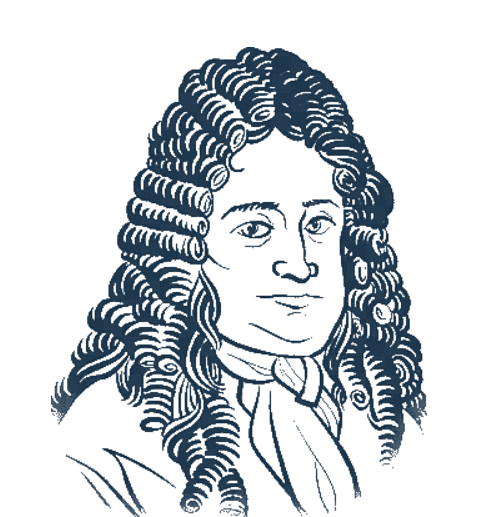
\includegraphics[width=0.5\linewidth]{figures/leibniz_photo.png}
            \captionof{figure}{Gottfried Wilhelm Leibniz}
        \end{center}
    }
    
    \block{Step Reckoner Calculating Machine}{
        \begin{center}
            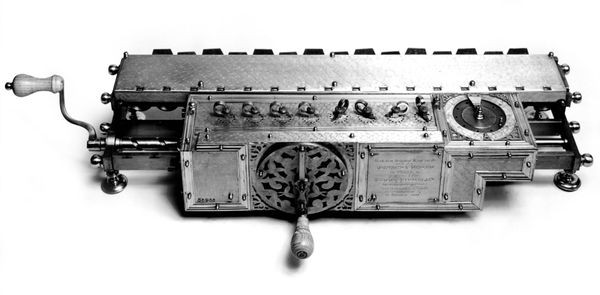
\includegraphics[width=0.8\linewidth]{figures/Step_Reckoner.jpg}
            \captionof{figure}{The Leibniz Step Reckoner}
        \end{center}
        
        \vspace{1cm}
    
        Leibniz, during his time in Paris in the early 1670s, came across Pascal's calculating machine known as the Pascaline. However, he saw its limitations, as it could only perform addition and subtraction operations. He became interested in enhancing the machine to include multiplication, division, and faster calculations.
        
        In 1672, Leibniz began working on his own calculating machine and completed it in 1694. Named the Step Reckoner, it far surpassed the capabilities of the Pascaline, as it could perform all four arithmetic operations mechanically. Leibniz presented a metallic version of his machine to the French Academy of Sciences in 1675.

        Leibniz's calculating machine utilized a counting device called the Leibniz wheel or stepped cylinder. This mechanism allowed each gear to represent a decimal digit from zero to nine in a single revolution, making it a dominant approach in calculating machine design for the next two centuries. 
        
        The Step Reckoner consisted of an accumulator capable of holding 16 decimal digits and an 8-digit input section. The machine operated by adding or subtracting the operands from the accumulator as many times as necessary. It could add or subtract an 8-digit number to/from the 16-digit accumulator, multiply two 8-digit numbers, and divide a 16-bit number by an 8-digit number. Addition and subtraction were performed in a single step, with the operating crank turned in the opposite direction for subtraction. The resulting calculation was stored in the accumulator.

        Leibniz demonstrated a prototype of his incomplete machine to the Royal Society in London during his visit in 1673, where he had the chance to meet with renowned scientists like Hooke and Boyle. 
        
        Leibniz's invention revolutionized calculation capabilities and laid the foundation for future calculating machines for the following 200 years.
        }


    \column{0.5}
    \block{Binary Numbers}{
        Arithmetic has traditionally been done using decimal notation, with digits ranging from 0 to 9. Leibniz recognized the potential of the binary number system, which uses only the digits 0 and 1. 
        
        In this system, the number two is represented as 10, four is represented as 100, and so on. Leibniz explained the binary system in his 1703 paper, "Explication de l'Arithmetique Binaire." He discussed how binary numbers can be added, subtracted, multiplied, and divided, emphasizing their advantages. 
        
        The key advantage of binary notation lies in digital computers, where a binary digit can be represented by an on-off switch. 
        
        Claude Shannon later demonstrated in his Master's thesis that these binary digits can be represented by electrical switches. This breakthrough allowed for binary arithmetic and more complex mathematical operations to be performed by relay circuits, forming the basis of digital computing. 
        \begin{center}
            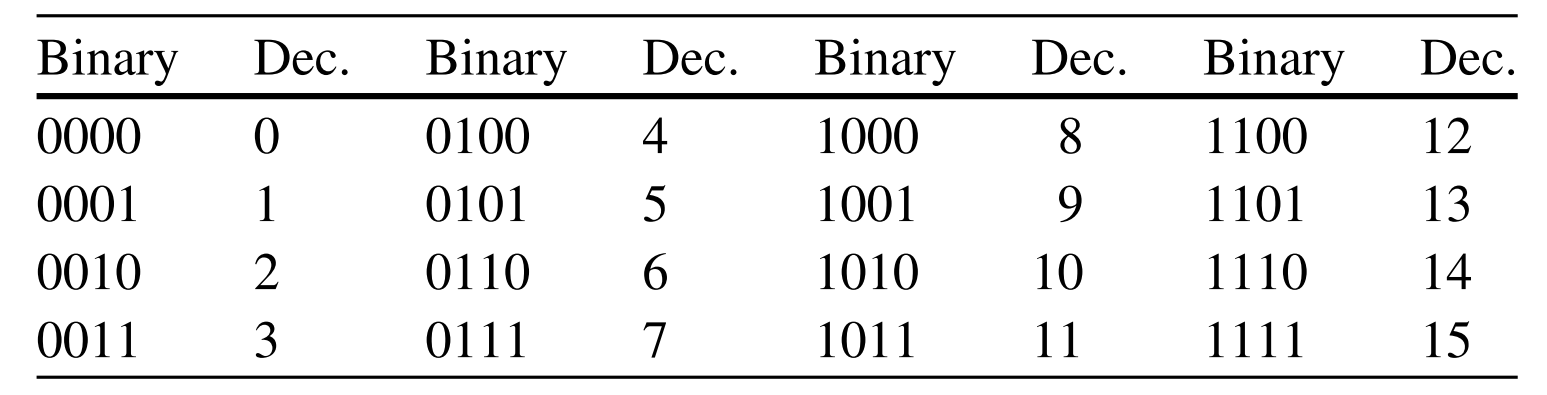
\includegraphics[width=0.9\linewidth]{figures/binary.png}
            \captionof{figure}{Binary number system}
        \end{center}
        }

    \block{Differential and Integral Calculus}{
    Differential calculus is the study of motion and acceleration, while integral calculus is used for problems related to area and volume. It is a significant field in mathematics that was developed independently by both Leibniz and Newton. The dispute over who truly first developed calculus resulted in controversy between the two mathematicians. It is now generally accepted that both Newton and Leibniz independently made their own contributions to calculus. Their work on calculus began in the late 17th century and demonstrated its practical applications in physics. Leibniz's notation introduced the dy/dx notation in differential calculus and the \(\int_{}^{} f(x) \,dx\) notation in integral calculus. Leibniz started his calculus work in 1673 and made visits to England in 1673 and 1676, while Newton began his work in 1666 and had already developed a theory of tangents when Leibniz started his research. The controversy surrounding whether Leibniz had access to Newton's unpublished manuscripts during his visits to England remains a key aspect of the dispute. 
    
    Calculus finds numerous applications in fields such as science and astronomy, where differential calculus is used to solve problems related to motion, change, and determining the tangent to a curve, and integral calculus is used for computations involving area and volume. 
        \begin{center}
            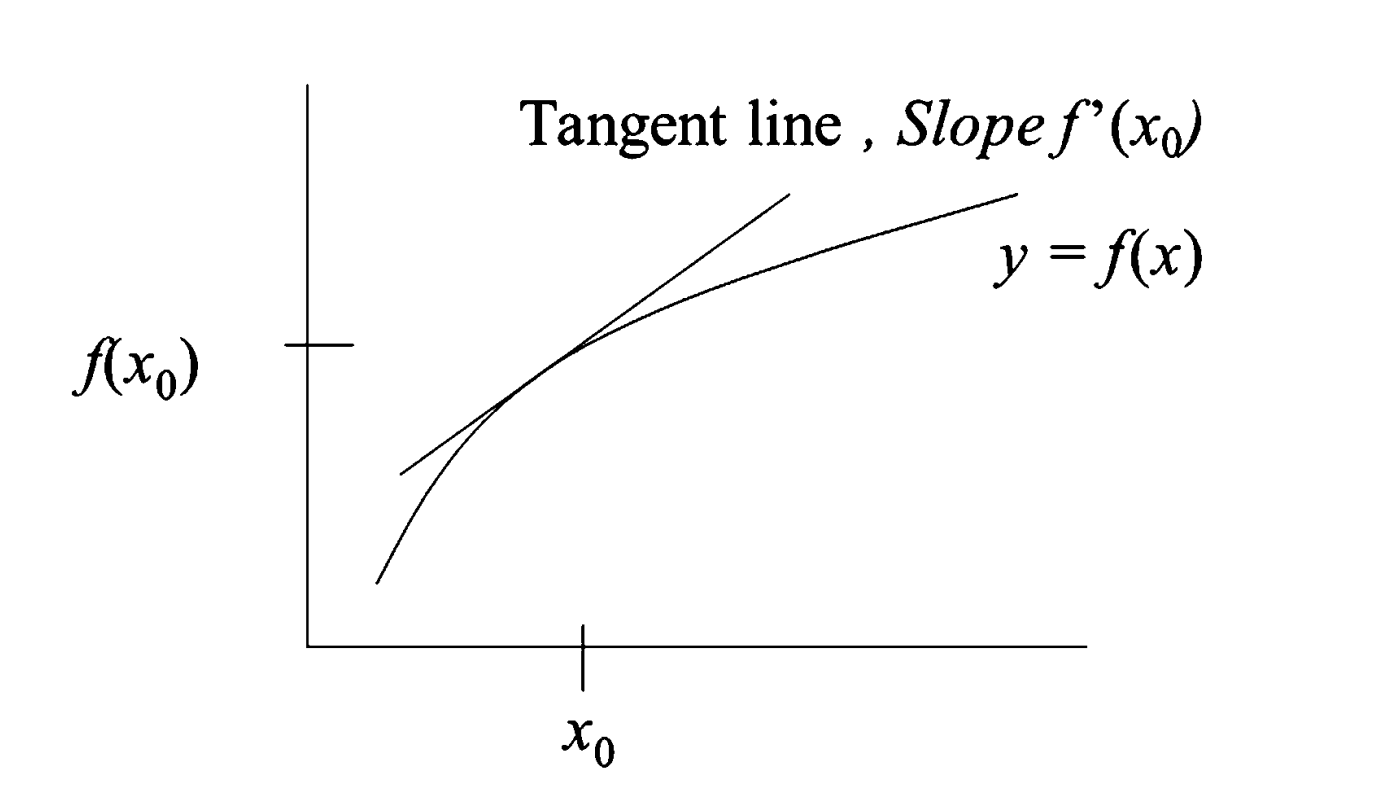
\includegraphics[width=0.6\linewidth]{figures/tangent_line.png}
        \end{center}
        }
    
    \block{Philosophy}{
    Leibniz's philosophy is centered around the concept of substance, where he posits the existence of countless monads. These monads, or souls, form an infinite family in Leibniz's rejection of the reality of matter. He argues that no causal relationship exists between two monads, and any appearance of such is illusory. Every monad reflects the universe, creating a hierarchy where some monads mirror with greater clarity. 
    
    The changes in one monad harmoniously correspond with those in another, simulating interaction. This analogous to synchronized clocks striking at the same time, with each clock functioning separately but perfectly. 
    
    Leibniz believes that space is not real, but rather an arrangement of monads in a three-dimensional order. He also introduces the principle of sufficient reason, asserting that nothing happens without a cause. Additionally, Leibniz presents arguments for the existence of God, building upon those previously formulated by Aristotle, St. Anselm, Aquinas, and Descartes, and improving their articulation.
        }

\end{columns}
\end{document}